\documentclass[11pt]{article}

\usepackage[margin=1in]{geometry}
\usepackage{graphicx}
\usepackage{fancyvrb}
\usepackage{minipage-marginpar}
\usepackage{changepage}

\newcommand{\fig}[2]{ 
\begin{figure}[h]
	\centering
	\caption{#2}
	\includegraphics[width=.75\textwidth]{pics/#1}
	\label{fig:#1}
\end{figure} 
}

\begin{document}

\title{CSCI 476: Lab 06}
\author{Nathan Stouffer}
\maketitle
\newpage

\section*{Task 1}

Task 1 asks us to familiarize ourselves with SQL statements. This is shown below in Figures \ref{fig:task1.1} and \ref{fig:task1.2}. Specifically, Figure \ref{fig:task1.1} shows opening mysql and Figure \ref{fig:task1.2} displays a command that views a specific row of the database.

\fig{task1.1}{Opening mysql}

\fig{task1.2}{Viewing a database entry}

\newpage 

\section*{Task 2}

In Task 2, we perform the SQL injection attack on a vulnerable website set up by SEED Labs. The vulnerable php code for the log in page is shown in Figure \ref{fig:task2.0}. The php code takes whatever is entered by the user and compiles it. This means a specially crafted input can change what is required to log in. This is shown in the subtasks below.

\fig{task2.0}{Vulnerable php code}

\subsection*{Task 2.1}

In Task 2.1, we are asked to log in as the administrator (with a username of admin) without knowing the password. This can be done by entering {\bf admin'; \#} in the username portion. This works since the database now ignores the password field and searches only for the username, which is admin. Figure \ref{fig:task2.2} shows the result of logging in as admin.

\fig{task2.1}{Logging in as admin on a webpage}

\fig{task2.2}{Showing admin result}

\subsection*{Task 2.2}

In Task 2.2, we perform the same attack as in Task 2.1 but from the command line instead of a webpage. This requires only a slight change in our attack strategy: we must now manually encode special characters such as whitespace and quotes. Figure \ref{fig:task2.3} shows an execution of the command and also redirects the output to a file called task2-out.html. We can then open the task2-out.html using a browser and see what we have in the output. This is shown in Figure \ref{fig:task2.4}. So we have the expected output of all the users!

\fig{task2.3}{Logging in as admin from command line}

\fig{task2.4}{Showing result}

\subsection*{Task 2.3}

Task 2.3 looks to chain multiple SQL statements together. SQL statements are separated only by a semicolon, so entering {\bf admin'; DELETE FROM credential WHERE Name='Alice'; \#} as the username in the log in page would login as admin and then delete the user Alice from the data base. I chose not to display a screenshot entering this since the username field on the webpage would not have shown the entire input. However, there is one issue: the above statement did not work (Figure \ref{fig:task2.5} displays the output of entering that as the username). This is because the php code uses a sql function that only allows an execution of one command. This is a step in the right direction from a protecting perspective.

\fig{task2.5}{Result of appending a second SQL statement}

\newpage 

\section*{Task 3}

Instead of just viewing information, Task 3 looks to update the data base with new values. In this task, we assume that we are a disgruntled employee named Alice. The subsequent subtasks show how we can use the SQL injection attack for malicious purposes. The attack is based on knowing the vulnerable php code in Figure \ref{fig:task3.0}.

\fig{task3.0}{Vulnerable php code}

\subsection*{Task 3.1}

Task 3.1 asks that we modify our own (Alice's) salary. Our first step is to log in as Alice, which we do using the technique form Task 2. Figure \ref{fig:task3.1} shows the login screen and Figure \ref{fig:task3.2} shows Alice's profile.

\begin{figure}[h]
	\centering
	\caption{Logging in as Alice}
	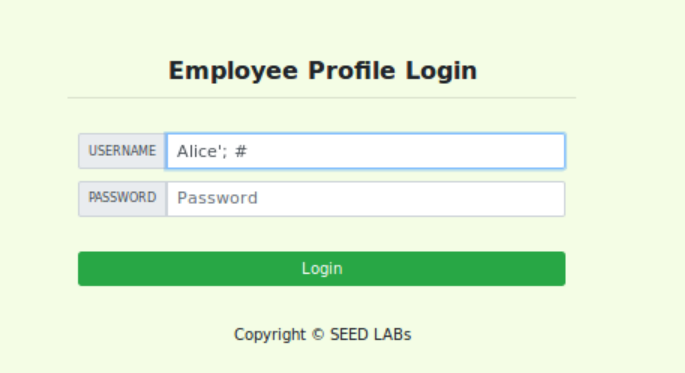
\includegraphics[width=.75\textwidth, height=4cm, keepaspectratio]{pics/task3.1}
	\label{fig:task3.1}
\end{figure}

%\fig{task3.1}{Logging in as Alice}

\fig{task3.2}{Alice's profile}

We then navigate to the edit profile page and enter {\bf ', salary=100000 WHERE Name=`Alice'; \#} in the nickname field. This command will change Alice's salary to 100000 and comment out the rest of the changes. The command is shown in Figure \ref{fig:task3.3} and the result can be seen in Figure \ref{fig:task3.4}.

\fig{task3.3}{Changing Alice's salary}

\fig{task3.4}{Showing new salary}

\subsection*{Task 3.2}

Task 3.2 asks us to modify other people's salary. We begin by again logging in as Alice and navigating to the edit profile page. Now, instead of entering {\bf ', salary=100000 WHERE Name=`Alice'; \#} in the nickname field, we enter {\bf ', salary=1 WHERE Name=`Boby'; \#} to change Boby's salary to \$1. The input is shown in Figure \ref{fig:task3.6} and the successful salary change is shown in Figure \ref{fig:task3.7} (I logged in as admin to view everyone's salary).

%\fig{task3.5}{arg2}

\fig{task3.6}{Changing Boby's salary}

\fig{task3.7}{Logged in as admin to view salaries}

\newpage

\subsection*{Task 3.3}

Task 3.3 asks that we modify Boby's password. We again do this from Alice's account on the edit profile page. However, changing a password is slightly different than updating salaries. We have to keep in mind that the password is hashed. A quick glance at the vulnerable php code in Figure \ref{fig:task3.0} shows that we can enter the password that we want into the new password field and then some malicious SQL statements in the Phone Number field to change whose password gets updated. Figure \ref{fig:task3.8} shows this where the SQL statement is {\bf ' WHERE Name=`Boby'; \#} and a new password is entered.

\fig{task3.8}{Changing Boby's password}

The above information gives the error shown in Figure \ref{fig:task3.9}, however, Boby's password does get updated (which can be seen in Figure \ref{fig:task3.11}).

\fig{task3.9}{Error message}

\newpage

Figure \ref{fig:task3.10} shows the login page for Boby and then Figure \ref{fig:task3.11} shows us successfully viewing Boby's profile.

\fig{task3.10}{Logging in as Boby}

\fig{task3.11}{Boby's profile}

\newpage 

\section*{Task 4}

Task 4 asks us to edit the code to make the website no longer vulnerable by using prepared statements. We do this for each of the vulnerable portions below. Figure \ref{fig:task4.1} shows the new code used for the log in page.

\fig{task4.1}{Updated login php code}

Figure \ref{fig:task4.2} displays the same login string that was passed in during Task 2, however, Figure \ref{fig:task4.3} shows that the attack is no longer successful and no such user is found.

\fig{task4.2}{Attempted SQL Injection}

\fig{task4.3}{Showing attack failure}

\newpage

We now give the edited code behind updating the profile (shown in Figure \ref{fig:task4.4}). This, again, uses prepared statements.

\fig{task4.4}{Updated edit profile code}

In Figure \ref{fig:task4.5}, we have logged in as Boby (since we know his password) and attempt to change his salary using the same attack described in Task 3. However, Figure \ref{fig:task4.6} shows that the attack no longer works. The salary is not updated and the exact string passed in for the Nickname field is now Boby's nickname.

\fig{task4.5}{Attempted SQL Injection}

\fig{task4.6}{Showing attack failure}

Overall, the SQL Injection attack is especially dangerous since an attacker does not need to know much information about the system. There is no need for figuring out what passwords are or even knowing a lot of user names (since they could try variations of admin). However, good software engineering standards, such as separating code and data, provide safe countermeasures against such attacks

\newpage 

\end{document}